\documentclass[10pt]{article}
\usepackage[a4paper,margin=23mm]{geometry}
\usepackage[T1]{fontenc}
\usepackage[utf8]{inputenc}
\usepackage{graphicx,booktabs,array,hyperref,microtype,pgfplots}
\pgfplotsset{compat=1.18}
\hypersetup{hidelinks,pdftitle={burn\_gekko: Camera Diagnostics and Stable Output Heads},pdfauthor={Mitchell Mosure}}
\setlength{\parindent}{0pt}\setlength{\parskip}{6pt}
\title{burn\_gekko: Camera Diagnostics and Stable Output Heads}\author{Mitchell Mosure}\date{Local technical draft / experiment pilot17-camera-diagnostics}
\begin{document}\maketitle
\begin{abstract}
One frozen multi-view foundation with its final trained camera-calibration and RGB heads. RGB completion remains 21.09 dB hidden-pixel PSNR on the 24-target synthetic head cohort. A new CPU diagnostic on 186 real TUM pairs reaches 14.19\% mean calibrated pose AUC at 10 degrees using five-point hypotheses across eight fixed solver seeds. The original eight-point protocol, all controls and failed transfer gates remain visible. Camera calibration still overfits; solver improvements do not establish new learned capability or resolved blur. This report presents a single selected training experiment in Burn, with fixed-teacher latent completion, co-visibility evaluation and declared correspondence readouts. Every table and visual binds to one checkpoint. Latent-space visualization is distinct from RGB synthesis; state-of-the-art performance is not established.
\end{abstract}
\section{Model and task}
An audited MIT V-JEPA 2.1 Base image encoder supplies final and block-6 features to six fusion blocks of width 384 with six attention heads. This phase starts from the audited own Pilot 12 checkpoint, resets both AdamW optimizers, and trains all 151 encoder tensors. Images are 256 by 256, batch size is 16, two references are provided and 90\% of target patches are masked. The original fixed V-JEPA supplies latent targets. A fixed own Pilot 11 encoder supplies training-only final-feature preservation with weight 4.0; it is absent from inference. The latent, RI and image-homography objectives are retained. Seed is 829, trunk learning rate is 2e-5, encoder rate is 4e-7, warmup is 32 and the cosine horizon is 384 updates. The spatial residual is bounded by 25\% of the centered block-6 norm. Matching uses a fixed 3 by 3 local probability centroid, plus the retained hard readout. An additional renderer-supervised bidirectional correspondence NLL has weight 0.1 and temperature 0.07. It pairs the dense target with a rotating reference using known visible patch-center projections. Source depth discontinuities, unknown depth, occlusion, out-of-frame and descriptor-border locations are excluded. Geometry supplies detached training labels only. All inference inputs are RGB. Known intrinsics enter the calibrated CPU pose solver after inference. No noncommercial pretrained weights or teachers are used. Attached RGB head: predicted 768-dimensional completion latent, 64-wide GELU MLP, sigmoid 16x16 RGB patches. Attached camera head: both directions of dense RGB-pair fusion, 4x4 spatial pooling per direction, shared 16-channel projection and 64-wide MLP; six rotation coordinates, signed translation direction and log normalized focal lengths. Camera labels and target RGB are loss/scoring targets only. Both heads are trained from scratch with separate AdamW optimizers; the foundation is frozen.

Sparse target tokens retain their original image-grid positions before encoder attention. Reference views are independently encoded. Fusion uses image-grid rotary position encodings and a shared reference role. No camera intrinsics, extrinsics or 3D rays enter this checkpoint. A fixed MIT V-JEPA 2.1 teacher supervises normalized latent targets; dense teacher features are used by the loss only. The full-target relative-improvement branch is evaluated separately from sparse completion.

\section{Experiment and data}
The selected checkpoint is \texttt{0639afa2e19d0e7a}. This phase completed 384 updates over 2048 configured cached training rooms, with 6144 logged target exposures covering 2048 unique rooms. Configurations, weight ancestry, dataset identities and the selected checkpoint hash are retained in the bundled machine-readable results. User inputs are TOML; metrics and prediction artifacts are typed native Rust exports. Pretrained noncommercial Gekko weights are excluded from this training lineage.

Completion evaluation role: \textbf{development}. Hidden-token MSE averages channels and hidden patches, then target views. Confidence intervals resample whole rooms rather than correlated pixels. The evaluation contains 512 target views. Evaluation geometry is loaded after inference to score co-visibility and correspondence; any training-room geometry supervision is declared separately above. Teacher-fitted display projections are visualization tools and do not enter inference or evaluation metrics.

\section{Optimization trajectory}
\begin{center}\resizebox{0.98\linewidth}{!}{\pgfplotsset{xmin=0,xmax=384,xtick={0,96,192,288,384}}
\begin{tikzpicture}
\begin{axis}[width=\linewidth,height=65mm,xlabel={Optimizer update},ylabel={Latent MSE},grid=major,scaled x ticks=false,legend style={at={(0.5,1.03)},anchor=south,legend columns=3,font=\scriptsize},tick label style={font=\small}]
\addplot[color=teal,mark=none,thick] table[x=step,y=cross,col sep=comma]{media/training.csv};
\addlegendentry{Cross-view train}
\addplot[color=orange,mark=none,thick] table[x=step,y=monocular,col sep=comma]{media/training.csv};
\addlegendentry{Monocular train}
\addplot[color=blue,dashed,mark=*,mark size=1.5pt] table[x=step,y=cross,col sep=comma]{media/validation.csv};
\addlegendentry{Validation cross}
\end{axis}
\end{tikzpicture}
}\end{center}
Training curves use nonoverlapping groups of at most 50 updates. Scheduled validation probes are shown when available. Every point belongs to this phase at or before the selected checkpoint. Validation uses development rooms and its declared masks; these curves do not establish independent generalization or training-seed convergence.
\section{How to read the metrics}
\paragraph{Calibrated camera-motion probe} A CPU geometric solver estimates motion from the model's matches and known intrinsics. Rotation and signed translation-direction errors use degrees; lower is better. Pose error is the larger angle. Pose AUC summarizes recall up to its angular threshold, displayed as a percentage; higher is better. Failed fits count as 180 degrees. Solver success means an estimate was returned, not that it was correct. This is separate from learned camera or focal-length prediction.
\paragraph{Feature signal / error (dB)} 10 log10(mean squared teacher feature / prediction MSE), measured on hidden patches and averaged over target views. Higher is better; +3.01 dB means half the error at the same signal power. It is not RGB PSNR and has no universal image-quality threshold.
\paragraph{RGB PSNR (dB)} 10 log10(RGB data range squared / RGB MSE). Reported only for an evaluated RGB decoder with a declared range, color space and mask. Colored feature plots cannot be scored as reconstructed images.
\paragraph{Feature MSE and cosine} MSE is mean squared feature error: zero is exact. Cosine measures feature-direction agreement: one is perfect alignment. A high cosine can coexist with lost spatial detail, so also inspect the variation ratio and shared-color feature maps.
\paragraph{Reference benefit (\%)} 100 times (1 - cross-view MSE / references-disabled MSE), using population means from the same checkpoint and targets. Positive means the reference images reduce error. Negative means they hurt.
\paragraph{Spatial variation retained (\%)} Predicted spatial feature variance divided by teacher variance. 100\% matches the teacher's amount of variation; lower values indicate smoothing. More than 100\% is not automatically better, and matched variance does not prove correct structure.
\paragraph{Mean match error (pixels)} AEPE: average distance between a predicted correspondence and its true position. Lower is better. HPatches uses the declared 240 by 240 scoring frame; ETH3D uses original image pixels. Neither is measured in the displayed thumbnail's pixels.
\paragraph{Within 3 pixels (\%)} PCK3: percentage of labeled matches whose error is at most three pixels in the declared scoring frame. Higher is better; 100\% is perfect. A gain of 1 percentage point means one additional match per hundred after the stated macro weighting.
\paragraph{Co-visibility ranking} AUROC compares visible and non-visible patches: 0.5 is chance and 1 is perfect. Average precision (AP) also depends on how many patches are visible, so read it alongside the positive-label fraction. These are ranking measures, not calibrated probabilities.
\paragraph{Known-transform loss (nats)} Negative log likelihood of the soft correspondence targets, using natural logarithms. Lower is better. Its scale depends on the grid, temperature and label distribution; compare it only within that fixed objective.
\paragraph{Camera and future heads} Rotation and translation-direction errors are angles in degrees (lower is better). Focal-length relative error can be shown as a percentage. Pose AUC reports accuracy over an angular threshold range. No camera, depth or RGB capability is claimed until that head is trained and evaluated.
\section{Absolute results for the selected checkpoint}
\subsection{Learned camera calibration head}
Head weights trained from scratch on a frozen foundation; Bevy anchor camera: +X right, +Y up, -Z forward; R maps target axes into reference axes; translation is reference-to-target direction in reference axes. Six-dimensional rotation columns, signed unit-baseline regression, log-positive focal lengths. No supplied calibration enters inference.
\begin{center}\begin{tabular}{p{.57\linewidth}rp{.23\linewidth}}\toprule Metric & Value & Unit / count \\ \midrule
Relative rotation error & 11.64 & degrees / 24 \\
Focal length relative error & 44.35 & \% / 24 \\
Signed translation-direction error & 32.68 & degrees / 24 \\
Pose AUC at 10 degrees & 3.18 & \% / 24 \\
\bottomrule\end{tabular}\end{center}
8 development rooms, 24 target/reference pairs; one training seed. Dense RGB pair input, independent from sparse completion. Principal point fixed at the image center; translation scale is not predicted. 0 invalid rotations; 0 focal clamps.

Training-label constant control: rotation 13.54 degrees, translation 85.29 degrees, focal error 45.64\%. Stable regression alone does not prove useful camera estimation.

\subsection{Learned RGB reconstruction head}
One trained 16x16 patch decoder shared by cross-view and references-disabled latent predictions. sRGB [0,1], data range 1, only originally hidden pixels scored; PSNR computed per view then averaged. Ground-truth pixels are never pasted into scored predictions.
\begin{center}\begin{tabular}{p{.57\linewidth}rp{.23\linewidth}}\toprule Metric & Value & Unit / count \\ \midrule
Hidden-pixel RGB PSNR & 21.09 & dB / 24 \\
References-disabled RGB PSNR & 20.70 & dB / 24 \\
Hidden-pixel RGB MSE & 0.0089 & squared sRGB units / 24 \\
\bottomrule\end{tabular}\end{center}
8 development rooms; fixed foundation and one head-training seed. This small head study does not establish sharp completion or real-scene transfer. Colored latent maps elsewhere remain feature visualizations.

\subsection{Camera and RGB training stability}
PASSED: fixed schedule, independent optimizers, warmup, global gradient clipping at 1 per head, finite-value checks and saved-weight replay. Failed gates: []. Final checkpoint only; no validation selection.
\begin{center}\begin{tabular}{p{.57\linewidth}rp{.23\linewidth}}\toprule Metric & Value & Unit / count \\ \midrule
Maximum camera gradient norm before clipping & 4.1301 & L2 norm / 800 \\
Maximum RGB gradient norm before clipping & 0.0545 & L2 norm / 800 \\
\bottomrule\end{tabular}\end{center}
Frozen-feature CPU phase: 800 updates in 64.7 seconds. Initial/final validation RGB PSNR 13.46/21.09 dB; camera regression loss 0.6206/0.3874. This verifies bounded optimization, not full encoder/fusion joint-training stability.

\subsection{Cross-view latent completion}
development; hidden tokens only, fixed V-JEPA 2.1 teacher, equal target-view weighting
\begin{center}\begin{tabular}{p{.57\linewidth}rp{.23\linewidth}}\toprule Metric & Value & Unit / count \\ \midrule
Feature signal / error (higher is better) & 7.38 & dB / 512 \\
Error reduction from reference views & 7.18 & \% / 512 \\
Hidden-token MSE & 0.1843 & squared normalized feature units / 512 \\
Hidden-token cosine & 0.9026 & cosine / 512 \\
Teacher spatial variation retained (100\% is reference) & 43.56 & \% / 512 \\
\bottomrule\end{tabular}\end{center}
Feature colors visualize latent space; they are not RGB reconstructions.

\subsection{Information-use controls}
Same checkpoint and masked targets as completion; only available reference information changes. Compare these MSE values with cross-view completion above.
\begin{center}\begin{tabular}{p{.57\linewidth}rp{.23\linewidth}}\toprule Metric & Value & Unit / count \\ \midrule
References disabled & 0.1986 & MSE / 512 \\
Reference positions shuffled & 0.1940 & MSE / 512 \\
Unrelated reference room & 0.2420 & MSE / 512 \\
Training-set mean at each position & 0.3084 & MSE / 512 \\
\bottomrule\end{tabular}\end{center}
Controls measure information use within this experiment; they are not separately trained model versions.

\subsection{Completion by reference visibility}
Post-hoc descriptive breakdown using geometry loaded after inference. Counts are hidden patches; errors are token-weighted, unlike the primary equal-view aggregate.
\begin{center}\begin{tabular}{p{.57\linewidth}rp{.23\linewidth}}\toprule Metric & Value & Unit / count \\ \midrule
Majority not visible: feature MSE & 0.1960 & MSE / 26243 \\
Majority visible in references: feature MSE & 0.1809 & MSE / 91472 \\
\bottomrule\end{tabular}\end{center}
A binary majority label does not mean every pixel in the patch is visible or occluded. This is a diagnostic, not a registered acceptance gate or a causal explanation of smoothing.

\subsection{Co-visibility}
hidden patches only; at least 128 known pixels; majority visible in any reference; ties counted visible; these evaluation co-visibility labels never supervise training. Separate training-room patch-center correspondences supervise the renderer auxiliary; they use a different labeling policy and no evaluation rooms. Geometry is never a model input.
\begin{center}\begin{tabular}{p{.57\linewidth}rp{.23\linewidth}}\toprule Metric & Value & Unit / count \\ \midrule
RI AUROC & 0.7382 & AUROC / 117715 \\
RI average precision & 0.9074 & AP / 117715 \\
\bottomrule\end{tabular}\end{center}
RI uses a separate full-target branch; it is not sparse completion.

Positive prevalence 77.7\%; AP depends on this prevalence.

\subsection{HPatches correspondence}
development; HP-240; pair then sequence means; primary viewpoint subset; patch-grid displacement
\begin{center}\begin{tabular}{p{.57\linewidth}rp{.23\linewidth}}\toprule Metric & Value & Unit / count \\ \midrule
Pair-conditioned descriptor  /  Mean match error & 15.67 & pixels / 295 \\
Pair-conditioned descriptor  /  Within 3 pixels & 15.53 & \% / 295 \\
Pair-conditioned descriptor + local refinement  /  Mean match error & 14.84 & pixels / 295 \\
Pair-conditioned descriptor + local refinement  /  Within 3 pixels & 26.23 & \% / 295 \\
Same-image conditioned control  /  Mean match error & 19.58 & pixels / 295 \\
Same-image conditioned control  /  Within 3 pixels & 13.42 & \% / 295 \\
Same-image conditioned control + local refinement  /  Mean match error & 18.90 & pixels / 295 \\
Same-image conditioned control + local refinement  /  Within 3 pixels & 21.29 & \% / 295 \\
Encoder block 6 control  /  Mean match error & 19.98 & pixels / 295 \\
Encoder block 6 control  /  Within 3 pixels & 13.39 & \% / 295 \\
Encoder block 6 control + local refinement  /  Mean match error & 19.33 & pixels / 295 \\
Encoder block 6 control + local refinement  /  Within 3 pixels & 20.33 & \% / 295 \\
\bottomrule\end{tabular}\end{center}
Local patch-grid readouts; optional 3x3 refinement is declared per method. No parity with published refinement or SOTA claim.

Pair-conditioned descriptor: AEPE 95\% cluster interval [13.043, 18.740] pixels over 59 sequence clusters; 10,000 deterministic bootstrap replicates.

Pair-conditioned descriptor + local refinement: AEPE 95\% cluster interval [12.190, 17.942] pixels over 59 sequence clusters; 10,000 deterministic bootstrap replicates.

Same-image conditioned control: AEPE 95\% cluster interval [16.759, 22.916] pixels over 59 sequence clusters; 10,000 deterministic bootstrap replicates.

Same-image conditioned control + local refinement: AEPE 95\% cluster interval [16.042, 22.261] pixels over 59 sequence clusters; 10,000 deterministic bootstrap replicates.

Encoder block 6 control: AEPE 95\% cluster interval [17.363, 23.008] pixels over 59 sequence clusters; 10,000 deterministic bootstrap replicates.

Encoder block 6 control + local refinement: AEPE 95\% cluster interval [16.682, 22.372] pixels over 59 sequence clusters; 10,000 deterministic bootstrap replicates.

\subsection{hpatches: paired readout gate -- PASS}
Pair-conditioned descriptor relative to Encoder block 6 control; Positive favors candidate: control minus candidate AEPE, candidate minus control PCK3. Pair means, then equal groups within each scene/sequence, then cluster bootstrap. One checkpoint; no training-seed uncertainty.
\begin{center}\begin{tabular}{p{.57\linewidth}rp{.23\linewidth}}\toprule Metric & Value & Unit / count \\ \midrule
Mean pixel error reduction & 4.31 & pixels / 295 \\
Accuracy gain at 3 pixels & 2.1369 & percentage points / 295 \\
\bottomrule\end{tabular}\end{center}
Paired 95\% AEPE-gain interval [3.7844, 4.8579] pixels; PCK3-gain interval [1.831, 2.444] percentage points. 59 clusters, 10,000 deterministic draws.

Fusion transfer gate passes: the pixel-error reduction interval must be entirely positive and mean within-3-pixel accuracy must not decrease. This is not an equivalence test or evidence of general SOTA performance.

\subsection{hpatches: paired readout gate -- PASS}
Pair-conditioned descriptor relative to Same-image conditioned control; Positive favors candidate: control minus candidate AEPE, candidate minus control PCK3. Pair means, then equal groups within each scene/sequence, then cluster bootstrap. One checkpoint; no training-seed uncertainty.
\begin{center}\begin{tabular}{p{.57\linewidth}rp{.23\linewidth}}\toprule Metric & Value & Unit / count \\ \midrule
Mean pixel error reduction & 3.91 & pixels / 295 \\
Accuracy gain at 3 pixels & 2.1120 & percentage points / 295 \\
\bottomrule\end{tabular}\end{center}
Paired 95\% AEPE-gain interval [3.2984, 4.5906] pixels; PCK3-gain interval [1.821, 2.413] percentage points. 59 clusters, 10,000 deterministic draws.

Fusion transfer gate passes: the pixel-error reduction interval must be entirely positive and mean within-3-pixel accuracy must not decrease. This is not an equivalence test or evidence of general SOTA performance.

\subsection{hpatches: paired readout gate -- PASS}
Pair-conditioned descriptor + local refinement relative to Encoder block 6 control + local refinement; Positive favors candidate: control minus candidate AEPE, candidate minus control PCK3. Pair means, then equal groups within each scene/sequence, then cluster bootstrap. One checkpoint; no training-seed uncertainty.
\begin{center}\begin{tabular}{p{.57\linewidth}rp{.23\linewidth}}\toprule Metric & Value & Unit / count \\ \midrule
Mean pixel error reduction & 4.49 & pixels / 295 \\
Accuracy gain at 3 pixels & 5.9061 & percentage points / 295 \\
\bottomrule\end{tabular}\end{center}
Paired 95\% AEPE-gain interval [3.9566, 5.0364] pixels; PCK3-gain interval [5.280, 6.564] percentage points. 59 clusters, 10,000 deterministic draws.

Fusion transfer gate passes: the pixel-error reduction interval must be entirely positive and mean within-3-pixel accuracy must not decrease. This is not an equivalence test or evidence of general SOTA performance.

\subsection{hpatches: paired readout gate -- PASS}
Pair-conditioned descriptor + local refinement relative to Same-image conditioned control + local refinement; Positive favors candidate: control minus candidate AEPE, candidate minus control PCK3. Pair means, then equal groups within each scene/sequence, then cluster bootstrap. One checkpoint; no training-seed uncertainty.
\begin{center}\begin{tabular}{p{.57\linewidth}rp{.23\linewidth}}\toprule Metric & Value & Unit / count \\ \midrule
Mean pixel error reduction & 4.06 & pixels / 295 \\
Accuracy gain at 3 pixels & 4.9392 & percentage points / 295 \\
\bottomrule\end{tabular}\end{center}
Paired 95\% AEPE-gain interval [3.4311, 4.7396] pixels; PCK3-gain interval [4.363, 5.549] percentage points. 59 clusters, 10,000 deterministic draws.

Fusion transfer gate passes: the pixel-error reduction interval must be entirely positive and mean within-3-pixel accuracy must not decrease. This is not an equivalence test or evidence of general SOTA performance.

\subsection{hpatches: paired readout gate -- PASS}
Pair-conditioned descriptor + local refinement relative to Pair-conditioned descriptor; Positive favors candidate: control minus candidate AEPE, candidate minus control PCK3. Pair means, then equal groups within each scene/sequence, then cluster bootstrap. One checkpoint; no training-seed uncertainty.
\begin{center}\begin{tabular}{p{.57\linewidth}rp{.23\linewidth}}\toprule Metric & Value & Unit / count \\ \midrule
Mean pixel error reduction & 0.83 & pixels / 295 \\
Accuracy gain at 3 pixels & 10.7054 & percentage points / 295 \\
\bottomrule\end{tabular}\end{center}
Paired 95\% AEPE-gain interval [0.7636, 0.8993] pixels; PCK3-gain interval [9.489, 12.042] percentage points. 59 clusters, 10,000 deterministic draws.

Local precision gate passes: the within-3-pixel gain interval must be entirely positive and mean pixel error must not increase. This is not an equivalence test or evidence of general SOTA performance.

\subsection{ETH3D correspondence}
development; original pixels; pair then scene then interval means; patch-grid displacement
\begin{center}\begin{tabular}{p{.57\linewidth}rp{.23\linewidth}}\toprule Metric & Value & Unit / count \\ \midrule
Pair-conditioned descriptor  /  Mean match error & 27.20 & pixels / 3365 \\
Pair-conditioned descriptor  /  Within 3 pixels & 2.34 & \% / 3365 \\
Pair-conditioned descriptor + local refinement  /  Mean match error & 23.81 & pixels / 3365 \\
Pair-conditioned descriptor + local refinement  /  Within 3 pixels & 5.68 & \% / 3365 \\
Same-image conditioned control  /  Mean match error & 34.28 & pixels / 3365 \\
Same-image conditioned control  /  Within 3 pixels & 2.19 & \% / 3365 \\
Same-image conditioned control + local refinement  /  Mean match error & 31.52 & pixels / 3365 \\
Same-image conditioned control + local refinement  /  Within 3 pixels & 4.65 & \% / 3365 \\
Encoder block 6 control  /  Mean match error & 32.96 & pixels / 3365 \\
Encoder block 6 control  /  Within 3 pixels & 2.30 & \% / 3365 \\
Encoder block 6 control + local refinement  /  Mean match error & 30.57 & pixels / 3365 \\
Encoder block 6 control + local refinement  /  Within 3 pixels & 4.30 & \% / 3365 \\
\bottomrule\end{tabular}\end{center}
Local patch-grid readouts; optional 3x3 refinement is declared per method. No parity with published refinement or SOTA claim.

Pair-conditioned descriptor: AEPE 95\% cluster interval [22.922, 31.869] pixels over 10 scene clusters; 10,000 deterministic bootstrap replicates.

Pair-conditioned descriptor + local refinement: AEPE 95\% cluster interval [19.209, 28.804] pixels over 10 scene clusters; 10,000 deterministic bootstrap replicates.

Same-image conditioned control: AEPE 95\% cluster interval [29.145, 39.384] pixels over 10 scene clusters; 10,000 deterministic bootstrap replicates.

Same-image conditioned control + local refinement: AEPE 95\% cluster interval [26.177, 36.783] pixels over 10 scene clusters; 10,000 deterministic bootstrap replicates.

Encoder block 6 control: AEPE 95\% cluster interval [28.351, 37.521] pixels over 10 scene clusters; 10,000 deterministic bootstrap replicates.

Encoder block 6 control + local refinement: AEPE 95\% cluster interval [25.862, 35.253] pixels over 10 scene clusters; 10,000 deterministic bootstrap replicates.

\subsection{eth3d: paired readout gate -- PASS}
Pair-conditioned descriptor relative to Encoder block 6 control; Positive favors candidate: control minus candidate AEPE, candidate minus control PCK3. Pair means, then equal groups within each scene/sequence, then cluster bootstrap. One checkpoint; no training-seed uncertainty.
\begin{center}\begin{tabular}{p{.57\linewidth}rp{.23\linewidth}}\toprule Metric & Value & Unit / count \\ \midrule
Mean pixel error reduction & 5.76 & pixels / 3365 \\
Accuracy gain at 3 pixels & 0.0375 & percentage points / 3365 \\
\bottomrule\end{tabular}\end{center}
Paired 95\% AEPE-gain interval [4.3991, 7.3494] pixels; PCK3-gain interval [-0.008, 0.074] percentage points. 10 clusters, 10,000 deterministic draws.

Fusion transfer gate passes: the pixel-error reduction interval must be entirely positive and mean within-3-pixel accuracy must not decrease. This is not an equivalence test or evidence of general SOTA performance.

\subsection{eth3d: paired readout gate -- PASS}
Pair-conditioned descriptor relative to Same-image conditioned control; Positive favors candidate: control minus candidate AEPE, candidate minus control PCK3. Pair means, then equal groups within each scene/sequence, then cluster bootstrap. One checkpoint; no training-seed uncertainty.
\begin{center}\begin{tabular}{p{.57\linewidth}rp{.23\linewidth}}\toprule Metric & Value & Unit / count \\ \midrule
Mean pixel error reduction & 7.08 & pixels / 3365 \\
Accuracy gain at 3 pixels & 0.1497 & percentage points / 3365 \\
\bottomrule\end{tabular}\end{center}
Paired 95\% AEPE-gain interval [4.8046, 9.8022] pixels; PCK3-gain interval [0.106, 0.197] percentage points. 10 clusters, 10,000 deterministic draws.

Fusion transfer gate passes: the pixel-error reduction interval must be entirely positive and mean within-3-pixel accuracy must not decrease. This is not an equivalence test or evidence of general SOTA performance.

\subsection{eth3d: paired readout gate -- PASS}
Pair-conditioned descriptor + local refinement relative to Encoder block 6 control + local refinement; Positive favors candidate: control minus candidate AEPE, candidate minus control PCK3. Pair means, then equal groups within each scene/sequence, then cluster bootstrap. One checkpoint; no training-seed uncertainty.
\begin{center}\begin{tabular}{p{.57\linewidth}rp{.23\linewidth}}\toprule Metric & Value & Unit / count \\ \midrule
Mean pixel error reduction & 6.76 & pixels / 3365 \\
Accuracy gain at 3 pixels & 1.3807 & percentage points / 3365 \\
\bottomrule\end{tabular}\end{center}
Paired 95\% AEPE-gain interval [5.3285, 8.4300] pixels; PCK3-gain interval [1.085, 1.696] percentage points. 10 clusters, 10,000 deterministic draws.

Fusion transfer gate passes: the pixel-error reduction interval must be entirely positive and mean within-3-pixel accuracy must not decrease. This is not an equivalence test or evidence of general SOTA performance.

\subsection{eth3d: paired readout gate -- PASS}
Pair-conditioned descriptor + local refinement relative to Same-image conditioned control + local refinement; Positive favors candidate: control minus candidate AEPE, candidate minus control PCK3. Pair means, then equal groups within each scene/sequence, then cluster bootstrap. One checkpoint; no training-seed uncertainty.
\begin{center}\begin{tabular}{p{.57\linewidth}rp{.23\linewidth}}\toprule Metric & Value & Unit / count \\ \midrule
Mean pixel error reduction & 7.71 & pixels / 3365 \\
Accuracy gain at 3 pixels & 1.0377 & percentage points / 3365 \\
\bottomrule\end{tabular}\end{center}
Paired 95\% AEPE-gain interval [5.3247, 10.5373] pixels; PCK3-gain interval [0.786, 1.293] percentage points. 10 clusters, 10,000 deterministic draws.

Fusion transfer gate passes: the pixel-error reduction interval must be entirely positive and mean within-3-pixel accuracy must not decrease. This is not an equivalence test or evidence of general SOTA performance.

\subsection{eth3d: paired readout gate -- PASS}
Pair-conditioned descriptor + local refinement relative to Pair-conditioned descriptor; Positive favors candidate: control minus candidate AEPE, candidate minus control PCK3. Pair means, then equal groups within each scene/sequence, then cluster bootstrap. One checkpoint; no training-seed uncertainty.
\begin{center}\begin{tabular}{p{.57\linewidth}rp{.23\linewidth}}\toprule Metric & Value & Unit / count \\ \midrule
Mean pixel error reduction & 3.39 & pixels / 3365 \\
Accuracy gain at 3 pixels & 3.3444 & percentage points / 3365 \\
\bottomrule\end{tabular}\end{center}
Paired 95\% AEPE-gain interval [2.9974, 3.7744] pixels; PCK3-gain interval [2.806, 3.998] percentage points. 10 clusters, 10,000 deterministic draws.

Local precision gate passes: the within-3-pixel gain interval must be entirely positive and mean pixel error must not increase. This is not an equivalence test or evidence of general SOTA performance.

\subsection{Synthetic camera-view matching}
Fixed validation rooms, view 0 versus view 1, both directions. RGB-only predictions; renderer depth and camera labels enter scoring only. Pair, same-image and encoder controls share the query population.
\begin{center}\begin{tabular}{p{.57\linewidth}rp{.23\linewidth}}\toprule Metric & Value & Unit / count \\ \midrule
Centered encoder control / AEPE & 20.30 & pixels / 32 \\
Centered encoder control / PCK8 & 34.26 & \% / 32 \\
Centered encoder control / PCK16 & 63.32 & \% / 32 \\
Centered encoder control + local refinement / AEPE & 18.81 & pixels / 32 \\
Centered encoder control + local refinement / PCK8 & 41.98 & \% / 32 \\
Centered encoder control + local refinement / PCK16 & 67.20 & \% / 32 \\
Pair-conditioned descriptor / AEPE & 14.24 & pixels / 32 \\
Pair-conditioned descriptor / PCK8 & 43.97 & \% / 32 \\
Pair-conditioned descriptor / PCK16 & 76.75 & \% / 32 \\
Pair-conditioned descriptor + local refinement / AEPE & 12.18 & pixels / 32 \\
Pair-conditioned descriptor + local refinement / PCK8 & 58.72 & \% / 32 \\
Pair-conditioned descriptor + local refinement / PCK16 & 80.21 & \% / 32 \\
\bottomrule\end{tabular}\end{center}
Metrics continued.
\begin{center}\begin{tabular}{p{.57\linewidth}rp{.23\linewidth}}\toprule Metric & Value & Unit / count \\ \midrule
Same-image conditioned control / AEPE & 19.56 & pixels / 32 \\
Same-image conditioned control / PCK8 & 36.49 & \% / 32 \\
Same-image conditioned control / PCK16 & 65.61 & \% / 32 \\
Same-image conditioned control + local refinement / AEPE & 17.83 & pixels / 32 \\
Same-image conditioned control + local refinement / PCK8 & 46.01 & \% / 32 \\
Same-image conditioned control + local refinement / PCK16 & 69.84 & \% / 32 \\
\bottomrule\end{tabular}\end{center}
This is synthetic development evaluation. Training may use renderer-supervised correspondence labels; external real-image transfer is reported separately. Unknown, occluded, out-of-frame and grid-border queries are excluded under the pinned policy.

\subsection{Calibrated motion / Pair-conditioned descriptor + local refinement}
Evaluation role: development. TUM Freiburg 3 calibrated relative-motion diagnostic. RGB-only 256px model, fixed local centroid and mutual matches; known intrinsics supplied only to deterministic CPU eight-point essential RANSAC. Equal pair weight within sequence, then equal sequences. Failed fits contribute 180 degrees; ground-truth baselines below 1 cm excluded from translation/pose only. Not a learned camera head or official SLAM/relative-pose protocol.
\begin{center}\begin{tabular}{p{.57\linewidth}rp{.23\linewidth}}\toprule Metric & Value & Unit / count \\ \midrule
Solver success & 98.92 & \% / 186 \\
Mean rotation error & 7.78 & degrees / 186 \\
Mean signed translation-direction error & 52.80 & degrees / 185 \\
Pose AUC at 5 degrees & 1.54 & \% / 185 \\
Pose AUC at 10 degrees & 7.65 & \% / 185 \\
Pose AUC at 20 degrees & 18.86 & \% / 185 \\
Poses within 10 degrees & 21.10 & \% / 185 \\
\bottomrule\end{tabular}\end{center}
Known RGB intrinsics enter a CPU eight-point RANSAC solver after RGB-only model inference. This is not a trained camera head or predicted calibration.

Three sequences in one TUM environment; no official relative-pose benchmark parity or broad generalization claim. Failure counts and low-baseline exclusions remain explicit.

\subsection{Calibrated motion / Same-image conditioned control + local refinement}
Evaluation role: development. TUM Freiburg 3 calibrated relative-motion diagnostic. RGB-only 256px model, fixed local centroid and mutual matches; known intrinsics supplied only to deterministic CPU eight-point essential RANSAC. Equal pair weight within sequence, then equal sequences. Failed fits contribute 180 degrees; ground-truth baselines below 1 cm excluded from translation/pose only. Not a learned camera head or official SLAM/relative-pose protocol.
\begin{center}\begin{tabular}{p{.57\linewidth}rp{.23\linewidth}}\toprule Metric & Value & Unit / count \\ \midrule
Solver success & 98.39 & \% / 186 \\
Mean rotation error & 9.50 & degrees / 186 \\
Mean signed translation-direction error & 55.15 & degrees / 185 \\
Pose AUC at 5 degrees & 1.79 & \% / 185 \\
Pose AUC at 10 degrees & 6.54 & \% / 185 \\
Pose AUC at 20 degrees & 18.16 & \% / 185 \\
Poses within 10 degrees & 17.35 & \% / 185 \\
\bottomrule\end{tabular}\end{center}
Known RGB intrinsics enter a CPU eight-point RANSAC solver after RGB-only model inference. This is not a trained camera head or predicted calibration.

Three sequences in one TUM environment; no official relative-pose benchmark parity or broad generalization claim. Failure counts and low-baseline exclusions remain explicit.

\subsection{Calibrated motion / Encoder block 6 control + local refinement}
Evaluation role: development. TUM Freiburg 3 calibrated relative-motion diagnostic. RGB-only 256px model, fixed local centroid and mutual matches; known intrinsics supplied only to deterministic CPU eight-point essential RANSAC. Equal pair weight within sequence, then equal sequences. Failed fits contribute 180 degrees; ground-truth baselines below 1 cm excluded from translation/pose only. Not a learned camera head or official SLAM/relative-pose protocol.
\begin{center}\begin{tabular}{p{.57\linewidth}rp{.23\linewidth}}\toprule Metric & Value & Unit / count \\ \midrule
Solver success & 98.92 & \% / 186 \\
Mean rotation error & 8.78 & degrees / 186 \\
Mean signed translation-direction error & 56.31 & degrees / 185 \\
Pose AUC at 5 degrees & 1.78 & \% / 185 \\
Pose AUC at 10 degrees & 5.85 & \% / 185 \\
Pose AUC at 20 degrees & 16.92 & \% / 185 \\
Poses within 10 degrees & 16.79 & \% / 185 \\
\bottomrule\end{tabular}\end{center}
Known RGB intrinsics enter a CPU eight-point RANSAC solver after RGB-only model inference. This is not a trained camera head or predicted calibration.

Three sequences in one TUM environment; no official relative-pose benchmark parity or broad generalization claim. Failure counts and low-baseline exclusions remain explicit.

\subsection{Camera-motion transfer gate}
FAILED: AUC@10 must improve over both controls in every sequence, without lower overall solver success.
\begin{center}\begin{tabular}{p{.57\linewidth}rp{.23\linewidth}}\toprule Metric & Value & Unit / count \\ \midrule
Pose AUC@10 gain over Same-image conditioned control + local refinement & 1.1072 & percentage points / 3 \\
Pose AUC@10 gain over Encoder block 6 control + local refinement & 1.8020 & percentage points / 3 \\
\bottomrule\end{tabular}\end{center}
Only three related sequences; the gate is a bounded diagnostic, not a SOTA qualification.

\subsection{Calibrated solver diagnostic / 8-point hypotheses}
Frozen RGB predictions; recorded local centroid versus hard patch center, with identical mutual flags, all methods/pairs and every declared solver seed. Known calibration only. All fits precede and are independent of truth diagnostics; failed poses count as 180 degrees. Mean camera metrics weight pairs within sequence, sequences within seed, then every seed. Epipolar summaries weight eligible pairs equally. Eight-point mode verifies the original seed replay; five-point mode changes only the minimal hypothesis solver and RANSAC sample size/stopping exponent. Both modes retain the same final linear refit and cheirality. No best-seed/readout selection or new trained weights.
\begin{center}\begin{tabular}{p{.57\linewidth}rp{.23\linewidth}}\toprule Metric & Value & Unit / count \\ \midrule
Pair-conditioned: Pose AUC at 10 degrees & 7.99 & \% / 8 \\
Pair-conditioned: Rotation error & 7.94 & degrees / 8 \\
Pair-conditioned: Translation-direction error & 51.71 & degrees / 8 \\
Same-image: Pose AUC at 10 degrees & 6.79 & \% / 8 \\
Same-image: Rotation error & 9.20 & degrees / 8 \\
Same-image: Translation-direction error & 55.95 & degrees / 8 \\
Encoder: Pose AUC at 10 degrees & 7.27 & \% / 8 \\
Encoder: Rotation error & 9.04 & degrees / 8 \\
Encoder: Translation-direction error & 56.42 & degrees / 8 \\
\bottomrule\end{tabular}\end{center}
Repeated TUM development data, not independent qualification.

Ground-truth epipolar consistency is a necessary, not sufficient, condition for a correct correspondence; along-line errors can pass.

Sampling opportunity assumes the maximum trial budget and independent trials; it is not pose-success probability or an estimate of real correspondence precision.

Solver-seed ranges are sensitivity ranges, not scene or training uncertainty.

Hard and recorded labels change coordinate readout only; exported descriptor method IDs retain their original names.

This table shows the registered subpixel readout. All hard-coordinate ablations, seed ranges and failures remain in the pinned source reports. This is calibrated post-inference fitting, not a learned camera head or predicted intrinsics. Model and attached RGB-head weights are unchanged.

\subsection{Calibrated solver diagnostic / 5-point hypotheses}
Frozen RGB predictions; recorded local centroid versus hard patch center, with identical mutual flags, all methods/pairs and every declared solver seed. Known calibration only. All fits precede and are independent of truth diagnostics; failed poses count as 180 degrees. Mean camera metrics weight pairs within sequence, sequences within seed, then every seed. Epipolar summaries weight eligible pairs equally. Eight-point mode verifies the original seed replay; five-point mode changes only the minimal hypothesis solver and RANSAC sample size/stopping exponent. Both modes retain the same final linear refit and cheirality. No best-seed/readout selection or new trained weights.
\begin{center}\begin{tabular}{p{.57\linewidth}rp{.23\linewidth}}\toprule Metric & Value & Unit / count \\ \midrule
Pair-conditioned: Pose AUC at 10 degrees & 14.19 & \% / 8 \\
Pair-conditioned: Rotation error & 5.46 & degrees / 8 \\
Pair-conditioned: Translation-direction error & 35.50 & degrees / 8 \\
Same-image: Pose AUC at 10 degrees & 12.88 & \% / 8 \\
Same-image: Rotation error & 6.02 & degrees / 8 \\
Same-image: Translation-direction error & 41.72 & degrees / 8 \\
Encoder: Pose AUC at 10 degrees & 12.33 & \% / 8 \\
Encoder: Rotation error & 6.11 & degrees / 8 \\
Encoder: Translation-direction error & 44.44 & degrees / 8 \\
\bottomrule\end{tabular}\end{center}
Repeated TUM development data, not independent qualification.

Ground-truth epipolar consistency is a necessary, not sufficient, condition for a correct correspondence; along-line errors can pass.

Sampling opportunity assumes the maximum trial budget and independent trials; it is not pose-success probability or an estimate of real correspondence precision.

Solver-seed ranges are sensitivity ranges, not scene or training uncertainty.

Hard and recorded labels change coordinate readout only; exported descriptor method IDs retain their original names.

This table shows the registered subpixel readout. All hard-coordinate ablations, seed ranges and failures remain in the pinned source reports. This is calibrated post-inference fitting, not a learned camera head or predicted intrinsics. Model and attached RGB-head weights are unchanged.

\subsection{Depth / future decoders}
Register a checkpoint-bound head evaluation to populate this capability.
\textbf{No evaluated capability is claimed for this head.}
Completion room-bootstrap 95\% interval: [0.181129, 0.187492], 128 rooms, 10,000 deterministic replicates. This measures scene sampling uncertainty, not variation across training seeds.
Paired gain from using references (monocular MSE minus cross-view MSE): 0.014259, room-bootstrap 95\% interval [0.012480, 0.016027]. Positive values favor reference use.
\subsection{Camera motion by sequence}
TUM RGB-D data \cite{tum} is CC BY 4.0. These three sequences share one acquisition environment; prior exposure in encoder pretraining is not established. Known intrinsics enter the CPU solver only. Solver success counts estimates returned, including inaccurate ones. Failed fits contribute 180 degrees. Exclusions are baselines below 1 cm and affect translation/pose only.
\begin{center}\small\begin{tabular}{llrrrrr}\toprule Sequence & Readout & Solved/all & Rot. $^\circ$ & Trans. $^\circ$ & AUC@10 \% & Excl. \\ \midrule
Office & Fusion & 60/62 & 13.13 & 50.19 & 6.82 & 0 \\
Structure far & Fusion & 62/62 & 4.73 & 53.58 & 7.90 & 0 \\
Structure near & Fusion & 62/62 & 5.47 & 54.62 & 8.23 & 1 \\
Office & Same-image & 60/62 & 14.97 & 63.47 & 3.77 & 0 \\
Structure far & Same-image & 62/62 & 4.57 & 56.32 & 5.92 & 0 \\
Structure near & Same-image & 61/62 & 8.96 & 45.67 & 9.93 & 1 \\
Office & Encoder & 60/62 & 15.20 & 59.83 & 4.62 & 0 \\
Structure far & Encoder & 62/62 & 4.76 & 62.20 & 6.22 & 0 \\
Structure near & Encoder & 62/62 & 6.37 & 46.91 & 6.71 & 1 \\
\bottomrule\end{tabular}\end{center}
\section{Visual evaluation protocol}
Examples are evenly spaced over the exported sample identities, retaining the first and last. They are not selected by prediction quality. All displayed teacher features share one three-component PCA projection and teacher-derived 2nd--98th percentile color bounds; predictions use the identical projection and bounds. Color structure describes representation variation, not RGB texture reconstruction. Error maps use a fixed 0--1 scale (dark blue to teal to yellow to red), saturating above 1. Co-visibility truth uses teal for shared geometry, coral for non-visible patches and gray for observed/unknown patches. Camera-motion panels identify predicted matches and RANSAC inliers; these are not ground-truth correspondences.
\clearpage\section*{Learned RGB and camera examples}
\subsection*{RGB head / room 2609308192, view 0}
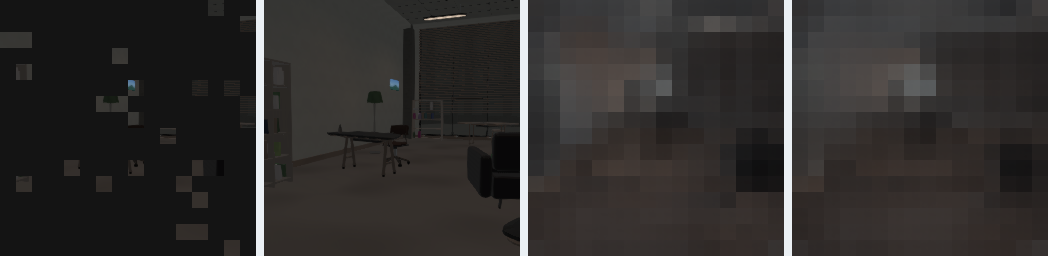
\includegraphics[width=.95\linewidth]{media/output-head-rgb-0.png}

Left to right: sparse target input, target RGB (evaluation only), predicted RGB, references-disabled RGB. Hidden-pixel PSNR 26.35 / 25.75 dB; the full images shown are generated by the same learned head. These fixed first/middle/last samples are not selected by quality.

\subsection*{Camera head / room 2609308192, view 0}
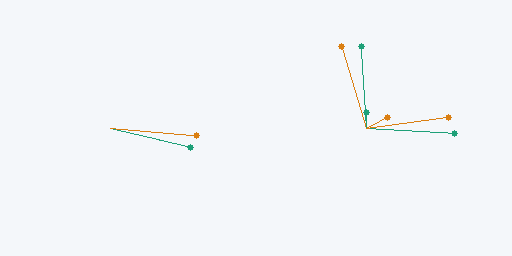
\includegraphics[width=.95\linewidth]{media/output-head-camera-0.png}

Green: renderer truth; amber: prediction. Left: signed unit translation; right: target orientation axes in the reference frame, under one fixed oblique projection. This is a dense RGB-pair route. Rotation error 19.15 degrees; translation-direction error 13.67 degrees; focal relative error 46.88\%. Diagram lengths are not metric translation scale.

\clearpage\section*{Learned RGB and camera examples}
\subsection*{RGB head / room 2609308196, view 0}

\includegraphics[width=.95\linewidth]{media/output-head-rgb-1.png}

Left to right: sparse target input, target RGB (evaluation only), predicted RGB, references-disabled RGB. Hidden-pixel PSNR 18.61 / 18.38 dB; the full images shown are generated by the same learned head. These fixed first/middle/last samples are not selected by quality.

\subsection*{Camera head / room 2609308196, view 0}
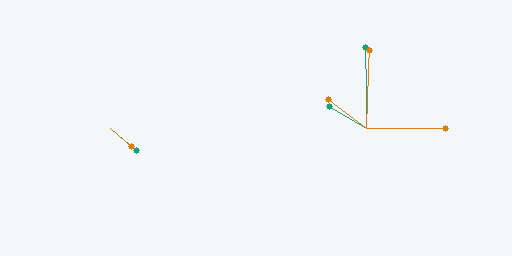
\includegraphics[width=.95\linewidth]{media/output-head-camera-1.png}

Green: renderer truth; amber: prediction. Left: signed unit translation; right: target orientation axes in the reference frame, under one fixed oblique projection. This is a dense RGB-pair route. Rotation error 4.75 degrees; translation-direction error 4.33 degrees; focal relative error 35.10\%. Diagram lengths are not metric translation scale.

\clearpage\section*{Learned RGB and camera examples}
\subsection*{RGB head / room 2609308199, view 2}

\includegraphics[width=.95\linewidth]{media/output-head-rgb-2.png}

Left to right: sparse target input, target RGB (evaluation only), predicted RGB, references-disabled RGB. Hidden-pixel PSNR 21.39 / 20.59 dB; the full images shown are generated by the same learned head. These fixed first/middle/last samples are not selected by quality.

\subsection*{Camera head / room 2609308199, view 2}
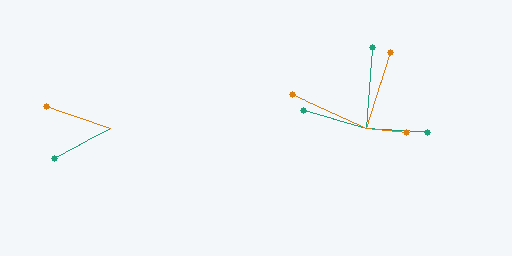
\includegraphics[width=.95\linewidth]{media/output-head-camera-2.png}

Green: renderer truth; amber: prediction. Left: signed unit translation; right: target orientation axes in the reference frame, under one fixed oblique projection. This is a dense RGB-pair route. Rotation error 19.98 degrees; translation-direction error 36.09 degrees; focal relative error 22.93\%. Diagram lengths are not metric translation scale.

\clearpage\section*{Geometric correspondence examples}
\subsection*{hpatches / v\_abstract\_2}
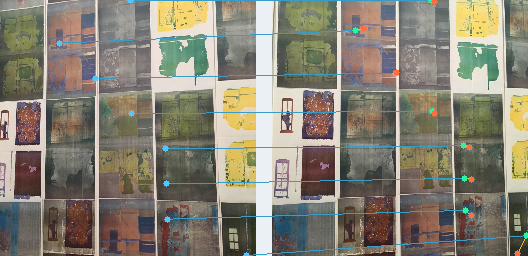
\includegraphics[width=.95\linewidth]{media/hpatches-matches-0.png}

Target left; reference right. Blue: target/true-match connection. Green: ground-truth reference location. Orange: model match. Yellow: matching error. Pair-conditioned descriptor + local refinement readout; mean match error 4.14 pixels in the 240 by 240 scoring frame. Eight labels selected uniformly, not by error. first/middle/last lexicographic pair in the primary subset; eight evenly spaced valid labels, no quality filtering.

\subsection*{hpatches / v\_gardens\_4}
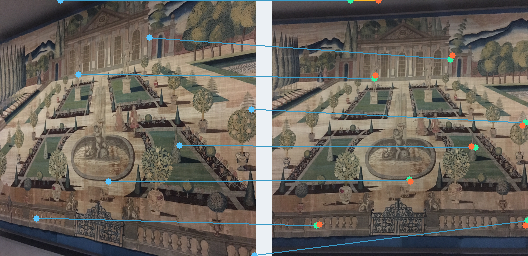
\includegraphics[width=.95\linewidth]{media/hpatches-matches-1.png}

Target left; reference right. Blue: target/true-match connection. Green: ground-truth reference location. Orange: model match. Yellow: matching error. Pair-conditioned descriptor + local refinement readout; mean match error 4.70 pixels in the 240 by 240 scoring frame. Eight labels selected uniformly, not by error. first/middle/last lexicographic pair in the primary subset; eight evenly spaced valid labels, no quality filtering.

\clearpage\section*{Geometric correspondence examples}
\subsection*{hpatches / v\_yuri\_6}
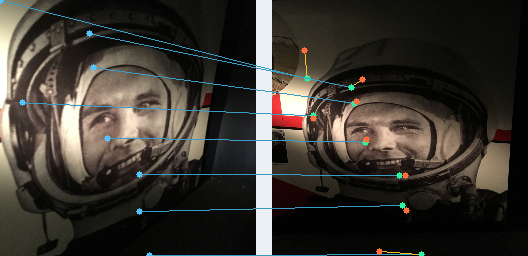
\includegraphics[width=.95\linewidth]{media/hpatches-matches-2.png}

Target left; reference right. Blue: target/true-match connection. Green: ground-truth reference location. Orange: model match. Yellow: matching error. Pair-conditioned descriptor + local refinement readout; mean match error 8.62 pixels in the 240 by 240 scoring frame. Eight labels selected uniformly, not by error. first/middle/last lexicographic pair in the primary subset; eight evenly spaced valid labels, no quality filtering.

\subsection*{eth3d / delivery\_area-11-0000}
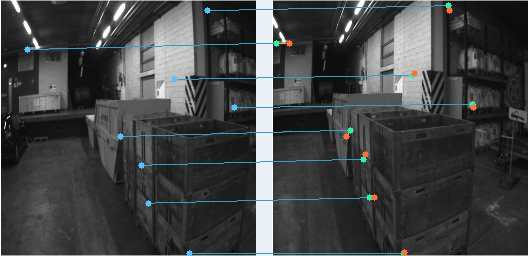
\includegraphics[width=.95\linewidth]{media/eth3d-matches-0.png}

Target left; reference right. Blue: target/true-match connection. Green: ground-truth reference location. Orange: model match. Yellow: matching error. Pair-conditioned descriptor + local refinement readout; mean match error 11.44 pixels in the 752 by 480 scoring frame. Eight labels selected uniformly, not by error. first/middle/last lexicographic pair in the primary subset; eight evenly spaced valid labels, no quality filtering.

\clearpage\section*{Geometric correspondence examples}
\subsection*{eth3d / playground-7-0015}
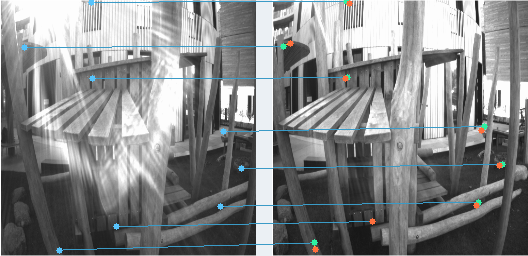
\includegraphics[width=.95\linewidth]{media/eth3d-matches-1.png}

Target left; reference right. Blue: target/true-match connection. Green: ground-truth reference location. Orange: model match. Yellow: matching error. Pair-conditioned descriptor + local refinement readout; mean match error 12.48 pixels in the 752 by 480 scoring frame. Eight labels selected uniformly, not by error. first/middle/last lexicographic pair in the primary subset; eight evenly spaced valid labels, no quality filtering.

\subsection*{eth3d / tunnel-9-0068}
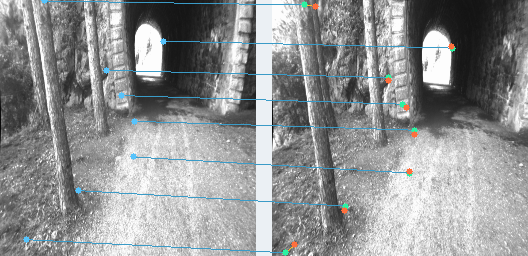
\includegraphics[width=.95\linewidth]{media/eth3d-matches-2.png}

Target left; reference right. Blue: target/true-match connection. Green: ground-truth reference location. Orange: model match. Yellow: matching error. Pair-conditioned descriptor + local refinement readout; mean match error 17.15 pixels in the 957 by 517 scoring frame. Eight labels selected uniformly, not by error. first/middle/last lexicographic pair in the primary subset; eight evenly spaced valid labels, no quality filtering.

\clearpage\section*{Geometric correspondence examples}
\subsection*{Actual camera views / room 2609308192}
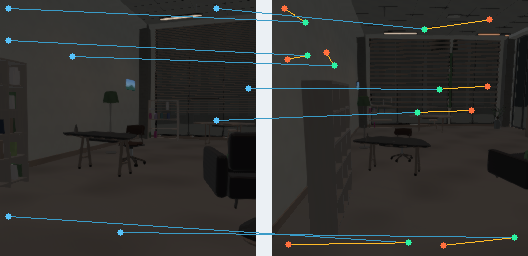
\includegraphics[width=.95\linewidth]{media/room-view-0.png}

View 0 left, view 1 right. Blue lines join source queries to renderer-projected green targets; orange marks RGB-model predictions and yellow shows error. Mean endpoint error 25.47 input pixels over all known visible queries. First four validation rooms; eight evenly spaced valid queries. Synthetic development data, not external transfer evidence.

\subsection*{Actual camera views / room 2609308193}
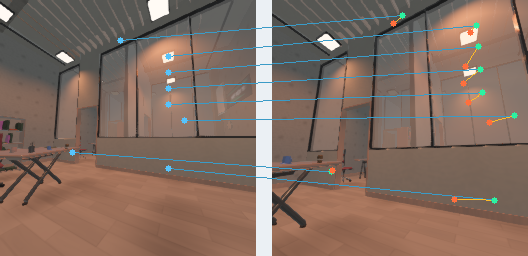
\includegraphics[width=.95\linewidth]{media/room-view-1.png}

View 0 left, view 1 right. Blue lines join source queries to renderer-projected green targets; orange marks RGB-model predictions and yellow shows error. Mean endpoint error 11.08 input pixels over all known visible queries. First four validation rooms; eight evenly spaced valid queries. Synthetic development data, not external transfer evidence.

\clearpage\section*{Geometric correspondence examples}
\subsection*{Actual camera views / room 2609308194}
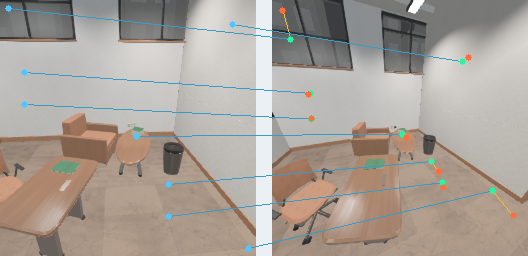
\includegraphics[width=.95\linewidth]{media/room-view-2.png}

View 0 left, view 1 right. Blue lines join source queries to renderer-projected green targets; orange marks RGB-model predictions and yellow shows error. Mean endpoint error 11.00 input pixels over all known visible queries. First four validation rooms; eight evenly spaced valid queries. Synthetic development data, not external transfer evidence.

\subsection*{Actual camera views / room 2609308195}
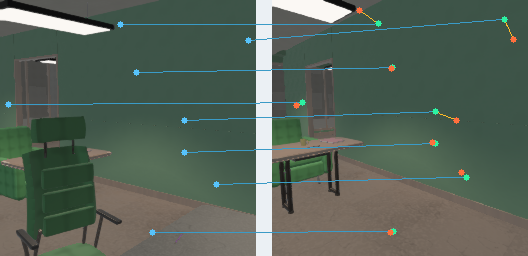
\includegraphics[width=.95\linewidth]{media/room-view-3.png}

View 0 left, view 1 right. Blue lines join source queries to renderer-projected green targets; orange marks RGB-model predictions and yellow shows error. Mean endpoint error 9.08 input pixels over all known visible queries. First four validation rooms; eight evenly spaced valid queries. Synthetic development data, not external transfer evidence.

\clearpage\section*{Geometric correspondence examples}
\subsection*{TUM camera motion / long\_office\_household-000081-000096}
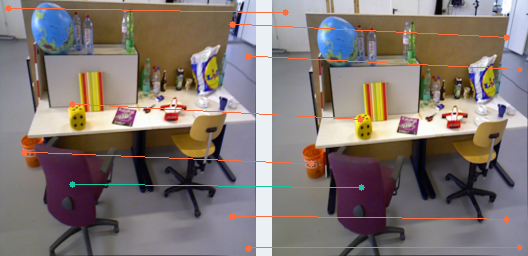
\includegraphics[width=.95\linewidth]{media/pose-00.png}

Target left; reference right. Model RGB input 256px; display thumbnails 256px. Predicted mutual correspondences: green marks RANSAC inliers, orange rejected matches. Inlier agreement is not ground-truth correctness. solver returned a pose; rotation error 3.20 degrees, signed translation-direction error 41.60 degrees. Known intrinsics enter the CPU solver only. first/middle/last lexicographic pair per sequence; up to eight uniformly spaced mutual matches, no quality filtering.

\subsection*{TUM camera motion / long\_office\_household-001302-001362}
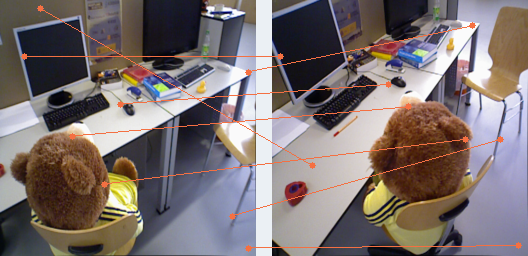
\includegraphics[width=.95\linewidth]{media/pose-01.png}

Target left; reference right. Model RGB input 256px; display thumbnails 256px. Predicted mutual correspondences: green marks RANSAC inliers, orange rejected matches. Inlier agreement is not ground-truth correctness. solver returned a pose; rotation error 11.44 degrees, signed translation-direction error 21.82 degrees. Known intrinsics enter the CPU solver only. first/middle/last lexicographic pair per sequence; up to eight uniformly spaced mutual matches, no quality filtering.

\clearpage\section*{Geometric correspondence examples}
\subsection*{TUM camera motion / long\_office\_household-002524-002584}
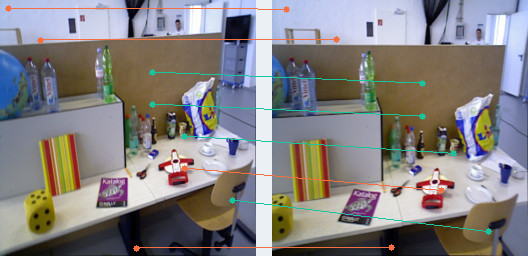
\includegraphics[width=.95\linewidth]{media/pose-02.png}

Target left; reference right. Model RGB input 256px; display thumbnails 256px. Predicted mutual correspondences: green marks RANSAC inliers, orange rejected matches. Inlier agreement is not ground-truth correctness. solver returned a pose; rotation error 2.16 degrees, signed translation-direction error 12.78 degrees. Known intrinsics enter the CPU solver only. first/middle/last lexicographic pair per sequence; up to eight uniformly spaced mutual matches, no quality filtering.

\subsection*{TUM camera motion / structure\_texture\_far-000028-000043}
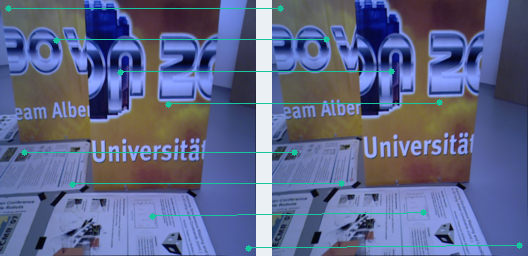
\includegraphics[width=.95\linewidth]{media/pose-03.png}

Target left; reference right. Model RGB input 256px; display thumbnails 256px. Predicted mutual correspondences: green marks RANSAC inliers, orange rejected matches. Inlier agreement is not ground-truth correctness. solver returned a pose; rotation error 1.70 degrees, signed translation-direction error 35.23 degrees. Known intrinsics enter the CPU solver only. first/middle/last lexicographic pair per sequence; up to eight uniformly spaced mutual matches, no quality filtering.

\clearpage\section*{Geometric correspondence examples}
\subsection*{TUM camera motion / structure\_texture\_far-000452-000512}
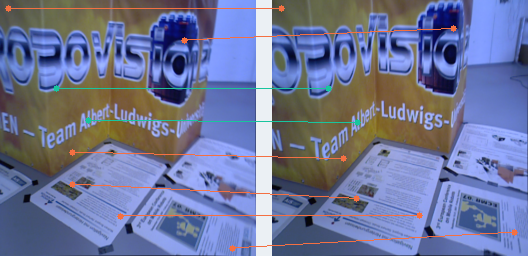
\includegraphics[width=.95\linewidth]{media/pose-04.png}

Target left; reference right. Model RGB input 256px; display thumbnails 256px. Predicted mutual correspondences: green marks RANSAC inliers, orange rejected matches. Inlier agreement is not ground-truth correctness. solver returned a pose; rotation error 10.61 degrees, signed translation-direction error 60.88 degrees. Known intrinsics enter the CPU solver only. first/middle/last lexicographic pair per sequence; up to eight uniformly spaced mutual matches, no quality filtering.

\subsection*{TUM camera motion / structure\_texture\_far-000877-000937}
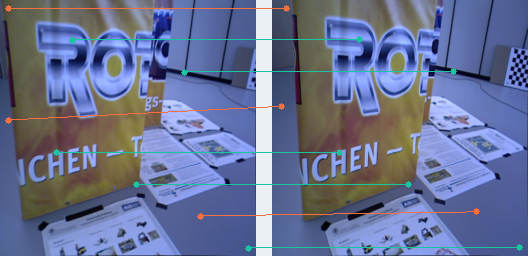
\includegraphics[width=.95\linewidth]{media/pose-05.png}

Target left; reference right. Model RGB input 256px; display thumbnails 256px. Predicted mutual correspondences: green marks RANSAC inliers, orange rejected matches. Inlier agreement is not ground-truth correctness. solver returned a pose; rotation error 3.50 degrees, signed translation-direction error 5.31 degrees. Known intrinsics enter the CPU solver only. first/middle/last lexicographic pair per sequence; up to eight uniformly spaced mutual matches, no quality filtering.

\clearpage\section*{Geometric correspondence examples}
\subsection*{TUM camera motion / structure\_texture\_near-000033-000048}
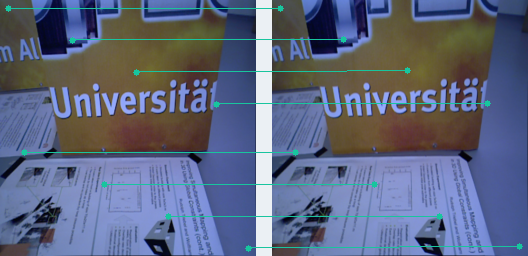
\includegraphics[width=.95\linewidth]{media/pose-06.png}

Target left; reference right. Model RGB input 256px; display thumbnails 256px. Predicted mutual correspondences: green marks RANSAC inliers, orange rejected matches. Inlier agreement is not ground-truth correctness. solver returned a pose; rotation error 0.50 degrees, signed translation-direction error excluded: baseline below 1 cm. Known intrinsics enter the CPU solver only. first/middle/last lexicographic pair per sequence; up to eight uniformly spaced mutual matches, no quality filtering.

\subsection*{TUM camera motion / structure\_texture\_near-000535-000595}
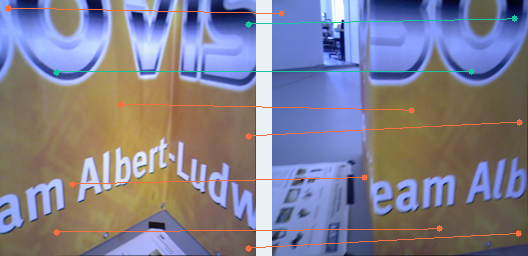
\includegraphics[width=.95\linewidth]{media/pose-07.png}

Target left; reference right. Model RGB input 256px; display thumbnails 256px. Predicted mutual correspondences: green marks RANSAC inliers, orange rejected matches. Inlier agreement is not ground-truth correctness. solver returned a pose; rotation error 22.02 degrees, signed translation-direction error 21.03 degrees. Known intrinsics enter the CPU solver only. first/middle/last lexicographic pair per sequence; up to eight uniformly spaced mutual matches, no quality filtering.

\clearpage\section*{Geometric correspondence examples}
\subsection*{TUM camera motion / structure\_texture\_near-001038-001098}
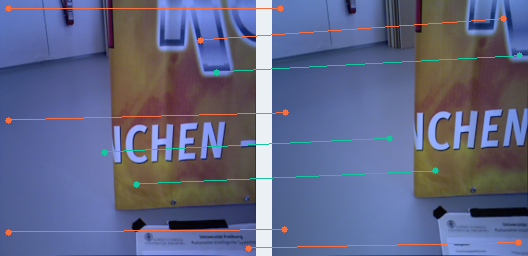
\includegraphics[width=.95\linewidth]{media/pose-08.png}

Target left; reference right. Model RGB input 256px; display thumbnails 256px. Predicted mutual correspondences: green marks RANSAC inliers, orange rejected matches. Inlier agreement is not ground-truth correctness. solver returned a pose; rotation error 4.66 degrees, signed translation-direction error 39.50 degrees. Known intrinsics enter the CPU solver only. first/middle/last lexicographic pair per sequence; up to eight uniformly spaced mutual matches, no quality filtering.

\clearpage\subsection{Room 2610091002, target view 0}
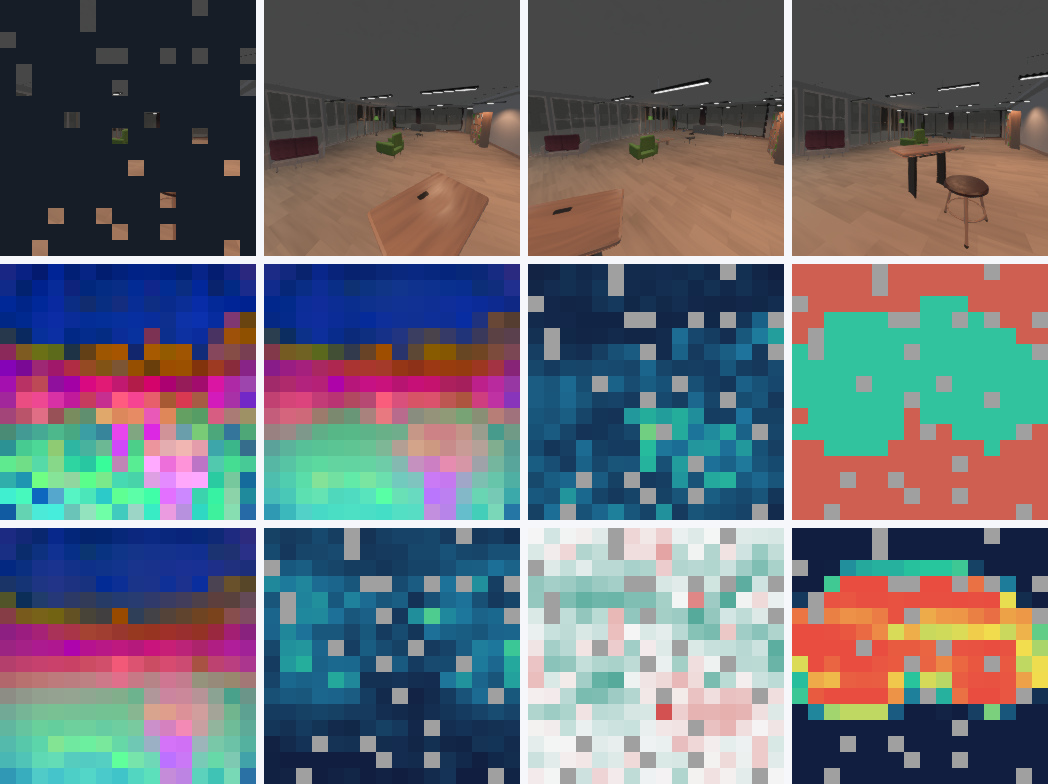
\includegraphics[width=\linewidth]{media/room-2610091002-view-0-sheet.png}

Top row, left to right: sparse target input; reference 1; reference 2 (or an explicitly blank panel); full target RGB for evaluation only. Second row: teacher latent; predicted latent; hidden-token error; geometric co-visibility truth. If present, the third row shows the same model's monocular latent, learned RI score, signed reference benefit and geometric visibility fraction. RI/fraction maps use a 0--1 scale. Reference benefit is (monocular MSE minus cross-view MSE) divided by monocular MSE: -1 red (worse), 0 white, +1 teal (better), saturating outside that range. Unlike the clipped training RI target, this display retains negative effects. RI is an unconstrained regression score, not a calibrated visibility probability. The teacher and full target do not enter sparse inference.

Feature signal/error: 8.66 dB (not RGB PSNR). Hidden-token MSE: 0.136011. Cosine: 0.928703. Values are recomputed in Rust from the exported arrays and checked against the population evaluation. All samples use the same error and projection conventions.
\clearpage\subsection{Room 2610091027, target view 2}
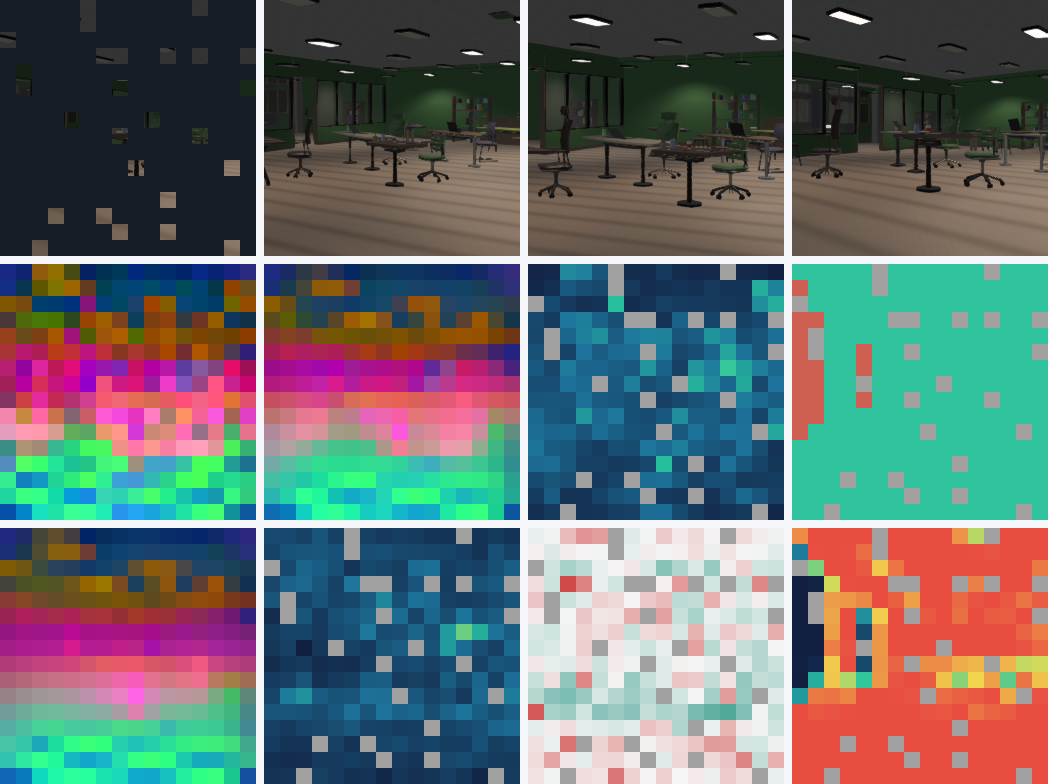
\includegraphics[width=\linewidth]{media/room-2610091027-view-2-sheet.png}

Top row, left to right: sparse target input; reference 1; reference 2 (or an explicitly blank panel); full target RGB for evaluation only. Second row: teacher latent; predicted latent; hidden-token error; geometric co-visibility truth. If present, the third row shows the same model's monocular latent, learned RI score, signed reference benefit and geometric visibility fraction. RI/fraction maps use a 0--1 scale. Reference benefit is (monocular MSE minus cross-view MSE) divided by monocular MSE: -1 red (worse), 0 white, +1 teal (better), saturating outside that range. Unlike the clipped training RI target, this display retains negative effects. RI is an unconstrained regression score, not a calibrated visibility probability. The teacher and full target do not enter sparse inference.

Feature signal/error: 7.69 dB (not RGB PSNR). Hidden-token MSE: 0.170213. Cosine: 0.910693. Values are recomputed in Rust from the exported arrays and checked against the population evaluation. All samples use the same error and projection conventions.
\clearpage\subsection{Room 2610091053, target view 0}
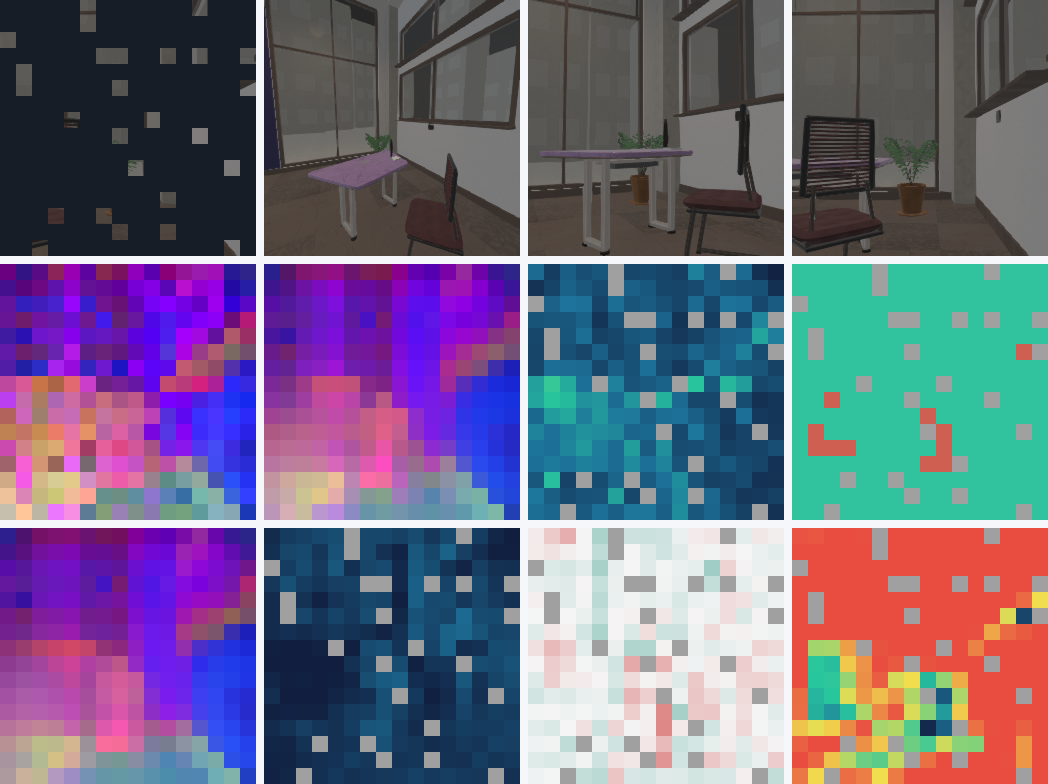
\includegraphics[width=\linewidth]{media/room-2610091053-view-0-sheet.png}

Top row, left to right: sparse target input; reference 1; reference 2 (or an explicitly blank panel); full target RGB for evaluation only. Second row: teacher latent; predicted latent; hidden-token error; geometric co-visibility truth. If present, the third row shows the same model's monocular latent, learned RI score, signed reference benefit and geometric visibility fraction. RI/fraction maps use a 0--1 scale. Reference benefit is (monocular MSE minus cross-view MSE) divided by monocular MSE: -1 red (worse), 0 white, +1 teal (better), saturating outside that range. Unlike the clipped training RI target, this display retains negative effects. RI is an unconstrained regression score, not a calibrated visibility probability. The teacher and full target do not enter sparse inference.

Feature signal/error: 7.07 dB (not RGB PSNR). Hidden-token MSE: 0.196250. Cosine: 0.895862. Values are recomputed in Rust from the exported arrays and checked against the population evaluation. All samples use the same error and projection conventions.
\clearpage\subsection{Room 2610091078, target view 2}
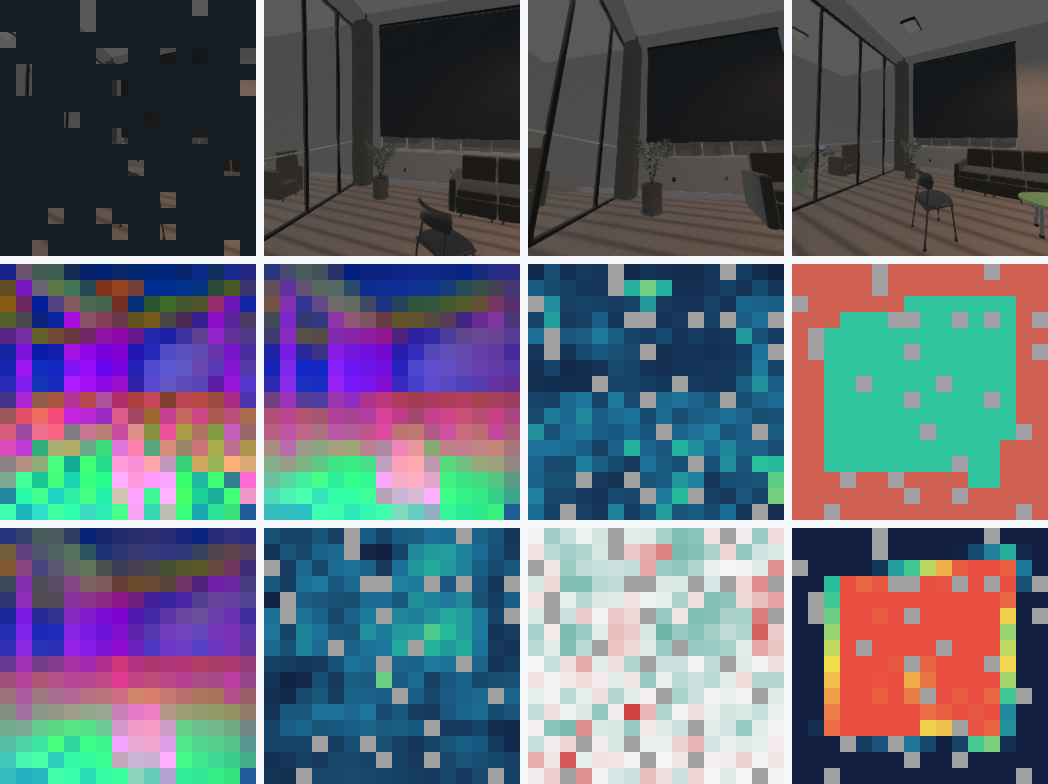
\includegraphics[width=\linewidth]{media/room-2610091078-view-2-sheet.png}

Top row, left to right: sparse target input; reference 1; reference 2 (or an explicitly blank panel); full target RGB for evaluation only. Second row: teacher latent; predicted latent; hidden-token error; geometric co-visibility truth. If present, the third row shows the same model's monocular latent, learned RI score, signed reference benefit and geometric visibility fraction. RI/fraction maps use a 0--1 scale. Reference benefit is (monocular MSE minus cross-view MSE) divided by monocular MSE: -1 red (worse), 0 white, +1 teal (better), saturating outside that range. Unlike the clipped training RI target, this display retains negative effects. RI is an unconstrained regression score, not a calibrated visibility probability. The teacher and full target do not enter sparse inference.

Feature signal/error: 7.91 dB (not RGB PSNR). Hidden-token MSE: 0.161992. Cosine: 0.914849. Values are recomputed in Rust from the exported arrays and checked against the population evaluation. All samples use the same error and projection conventions.
\clearpage\subsection{Room 2610091104, target view 0}
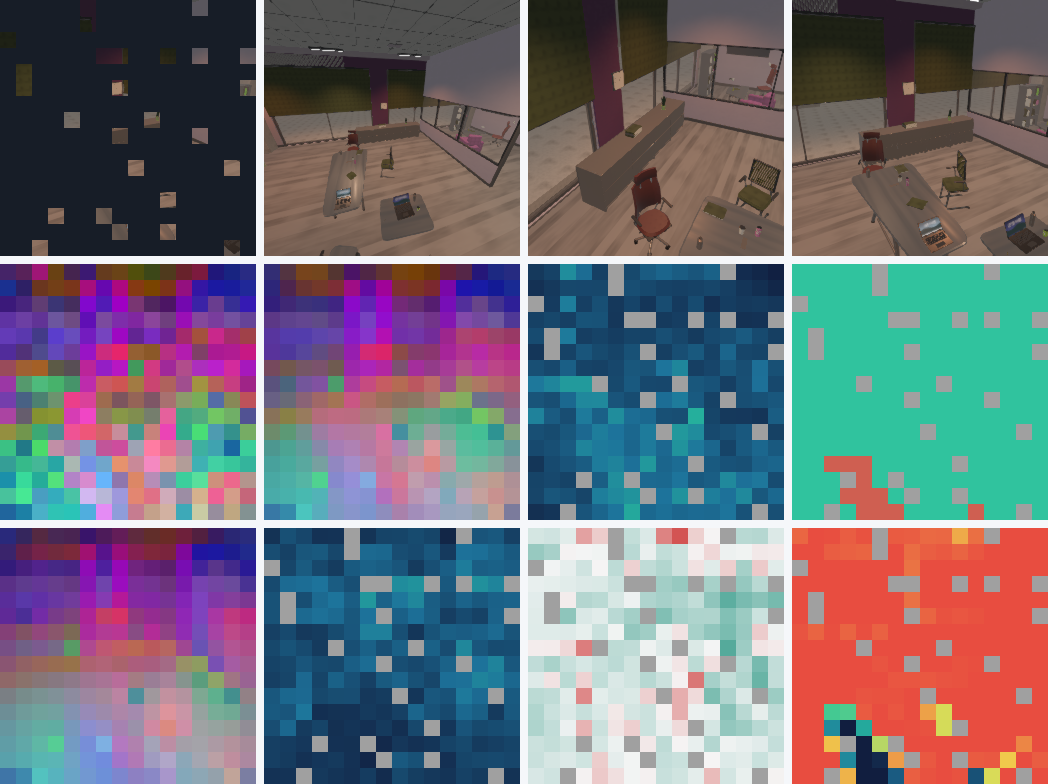
\includegraphics[width=\linewidth]{media/room-2610091104-view-0-sheet.png}

Top row, left to right: sparse target input; reference 1; reference 2 (or an explicitly blank panel); full target RGB for evaluation only. Second row: teacher latent; predicted latent; hidden-token error; geometric co-visibility truth. If present, the third row shows the same model's monocular latent, learned RI score, signed reference benefit and geometric visibility fraction. RI/fraction maps use a 0--1 scale. Reference benefit is (monocular MSE minus cross-view MSE) divided by monocular MSE: -1 red (worse), 0 white, +1 teal (better), saturating outside that range. Unlike the clipped training RI target, this display retains negative effects. RI is an unconstrained regression score, not a calibrated visibility probability. The teacher and full target do not enter sparse inference.

Feature signal/error: 7.67 dB (not RGB PSNR). Hidden-token MSE: 0.171015. Cosine: 0.909975. Values are recomputed in Rust from the exported arrays and checked against the population evaluation. All samples use the same error and projection conventions.
\clearpage\subsection{Room 2610091129, target view 3}
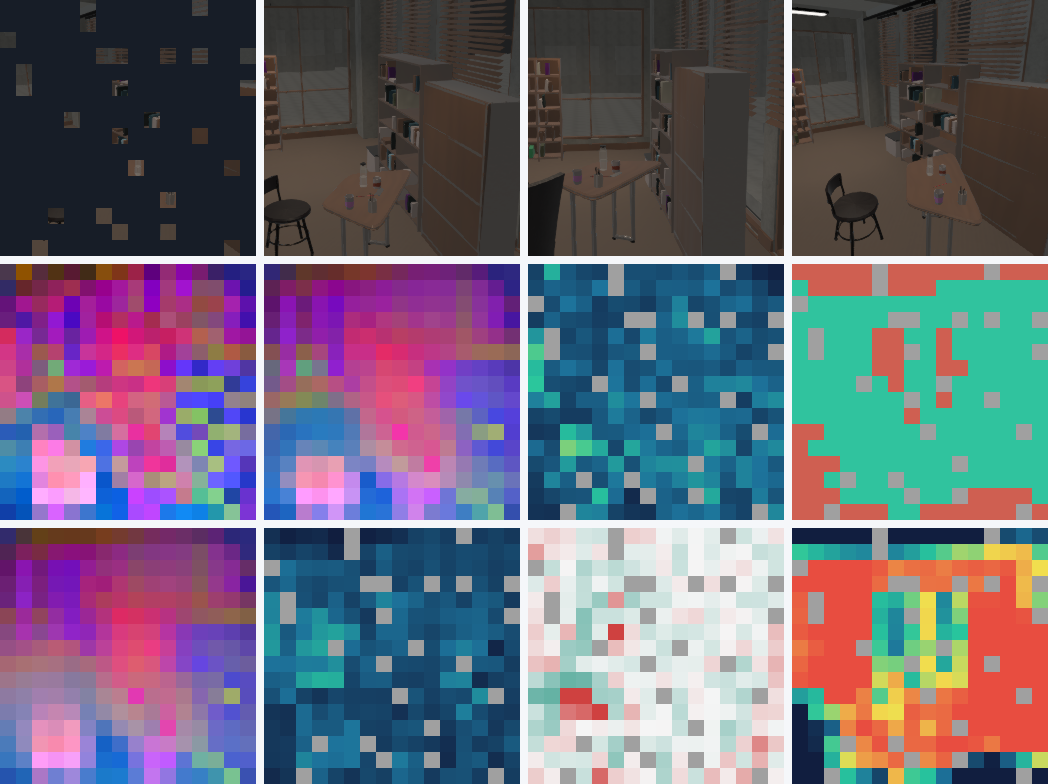
\includegraphics[width=\linewidth]{media/room-2610091129-view-3-sheet.png}

Top row, left to right: sparse target input; reference 1; reference 2 (or an explicitly blank panel); full target RGB for evaluation only. Second row: teacher latent; predicted latent; hidden-token error; geometric co-visibility truth. If present, the third row shows the same model's monocular latent, learned RI score, signed reference benefit and geometric visibility fraction. RI/fraction maps use a 0--1 scale. Reference benefit is (monocular MSE minus cross-view MSE) divided by monocular MSE: -1 red (worse), 0 white, +1 teal (better), saturating outside that range. Unlike the clipped training RI target, this display retains negative effects. RI is an unconstrained regression score, not a calibrated visibility probability. The teacher and full target do not enter sparse inference.

Feature signal/error: 6.92 dB (not RGB PSNR). Hidden-token MSE: 0.203265. Cosine: 0.892416. Values are recomputed in Rust from the exported arrays and checked against the population evaluation. All samples use the same error and projection conventions.
\section{Training efficiency}
Command duration 10.1 minutes; observed board energy 57.17 Wh; observed board joules per logged target 33.50; telemetry coverage 99.8\%. Device-wide board power/utilization, including shared desktop load; observed intervals only, gaps over 5 seconds excluded. Process memory is separately attributed. Stage timing excludes first 10 updates when at least 21 exist; energy retains command preparation and evaluation. Utilization is sample-median, not SM occupancy.
\begin{center}\begin{tabular}{lrrr}\toprule Encoder stage & Median (ms) & p95 (ms) & Targets/s \\ \midrule
2 & 1255.37 & 1302.47 & 12.75 \\
\bottomrule\end{tabular}\end{center}
Mean observed board power: 340.68 W. These are warmed per-update rates; complete-command energy retains preparation, validation and checkpoint overhead.
Peak training-process VRAM: 49110 MiB. Peak training-process RSS: 7285 MiB.

\paragraph{Encoder adaptation.} Verified training stages: 384 updates with full encoder trainable (steps 1-384). Logged encoder gradient counts are checked against each stage. These counts describe optimization, not evidence of improved transfer.

\paragraph{Encoder feature preservation.} Final encoder features are anchored to a pinned frozen ancestor with loss weight 4.0. Training feature RMS drift is 6.86\% in the first and 8.44\% in the last 32-update window (100 times the square root of mean per-image, energy-normalized feature MSE, equally weighted over sparse/full target and reference routes). Intermediate geometric features have no direct preservation target. This is a training regularization diagnostic, not RGB error or independent accuracy. The frozen anchor is absent from inference.

\paragraph{Renderer-supervised correspondence.} Renderer-supervised correspondence is a training-only auxiliary (weight 0.1, temperature 0.07). First versus last 32-update mean NLL: 2.768 to 2.419 nats; usable query fraction: 46.5\% to 47.1\%. These are changing-minibatch diagnostics. Geometry and camera labels are absent from RGB inference.
\paragraph{Training convergence diagnostic.} First versus last 32-update mean correspondence NLL: pair conditioning 1.5758 to 1.5008; same-image conditioning 1.6442 to 1.5560. These are descriptive minibatch statistics, not an independent generalization estimate. Known-transform descriptor supervision is motivated by SiLK \cite{silk}; implementation is independent, and no SiLK code or weights are used.
\clearpage\section{Limitations and qualification requirements}
\begin{itemize}
\item Pilot 17 adds CPU camera diagnostics for this same foundation checkpoint, with no new model or attached-head training. The 186 TUM pairs are reused development data. Five-point fitting uses known intrinsics after RGB inference and has a different solver protocol from the historical primary camera table. All methods, both coordinate readouts and all eight seeds are retained in pinned native reports. Fusion passes both control gates together in only one of eight solver seeds; this does not establish reliable transfer or SOTA.
\item This publication binds one frozen foundation checkpoint and one final attached-head training run. Head weight hashes, optimizer records, native validation predictions and training logs are pinned separately. It does not compare separately trained private model versions.
\item The 800-update head phase uses 32 training rooms and 8 disjoint validation rooms from existing synthetic data, with one seed. These are development cohorts previously used by the foundation study, not a fresh generalization test. The final checkpoint is fixed by the schedule, not chosen on validation performance.
\item Numerical head stability passed, but camera generalization is poor: training camera regression loss 0.000131 versus validation 0.387406; validation rotation 11.64 degrees, translation direction 32.68 degrees and focal relative error 44.35\%. The calibration head is not deployment-ready.
\item The camera head uses dense target/reference RGB pair features. RGB completion uses only sparse target and reference information. A centered principal point is assumed; translation scale is not predicted. No camera labels enter either inference path.
\item RGB PSNR uses hidden sRGB pixels in [0,1] and averages per-target PSNR. It is separate from feature signal/error dB. The same RGB decoder scores the cross-view and monocular routes. PSNR gains do not establish sharp details, geometric consistency or real-scene completion quality.
\item The latent gallery and external correspondence/solver results describe the unchanged foundation checkpoint. Attached-head metrics use a separate explicitly labeled 24-target cohort. Legacy calibrated RANSAC results use known intrinsics and are not measurements of the learned calibration head.
\item The training curve and board-efficiency panel describe the historical foundation phase. The attached heads train on CPU in 66.44 seconds total; frozen GPU feature export takes 44.99 seconds under the old remaining allowance. Desktop GPU activity is included in board observations. No process-attributed power claim.
\item A legacy assessment provenance flag incorrectly said geometry\_training\_supervision=false. Foundation training used renderer-supervised correspondence. The preserved training configuration and label-cache records are authoritative; the later exporter correction passed exact replay.
\item Encoder/fusion joint training with these output heads has not been qualified. Camera intrinsics generalization, additional seeds, larger datasets, strict numerical reference-order invariance, independent real data and matched public baselines remain open. SOTA and blur resolution are not established.
\item No noncommercial pretrained weights or teachers enter this lineage. Depth and other future heads remain untrained. Earlier recorded failed gates and numerical/exporter limitations are not waived by this head study.
\end{itemize}

\paragraph{Interactive demonstration.} \url{https://mosure.github.io/burn_gekko/demo/} runs this foundation checkpoint and its attached heads on live procedural Zeroverse rooms or two to four uploaded RGB photographs. Native and WebGPU paths share Rust inference and metric code. A dedicated worker keeps the scene editor responsive. Camera edits invalidate previous annotations. This demonstration uses new captures and is separate from the fixed offline evaluation protocol; RGB sharpness and camera generalization limitations remain.
\section{Reproducibility and extension}
The model library, trainer, data reader, evaluation and publication are separate Rust crates. A new decoder/head supplies a checkpoint-bound capability record with explicit metric units, population, aggregation and evaluation status. Camera scoring includes SO(3) angular error, signed translation-direction error, normalized focal error and pose AUC at 5, 10 and 20 degrees. Zero ground-truth baselines are excluded from translation-direction and pose denominators; a zero predicted translation at a valid baseline is a failure. A trained head requires the separate checkpoint-bound optimization and prediction evidence reported in its capability section.

Generate this page and report from one TOML experiment manifest with \texttt{gekko-report build}. The bundle carries input and output hashes, exact sample identities, a common latent projection and the resolved report data. Local preparation does not commit, push, deploy or upload the repository. Checkpoints from old code identities require their sealed binaries for exact optimizer resume; weights-only new phases must record explicit ancestry and optimizer resets.

\section{Related work and provenance}
The project studies sparse visual encoding and multi-view fusion motivated by V-JEPA 2.1 and Gekko. Procedural room captures use published bevy\_zeroverse packages. Calibrated 3D positional encodings remain a research extension. The optional supervised calibration head uses two continuous rotation columns, following the representation of Zhou et al. \cite{rotation6d}; it does not implement or claim the published camera systems referenced below.
The external matching protocols use the documented HPatches and ETH3D assets associated with ZeroCo \cite{zeroco}, with the local input resolution and readout explicitly declared. This is not reproduction of its complete published matching system.
\begin{thebibliography}{9}
\bibitem{vjepa21} L. Mur-Labadia et al. V-JEPA 2.1: Unlocking Dense Features in Video Self-Supervised Learning. \url{https://arxiv.org/abs/2603.14482v3}.
\bibitem{zeroverse} M. Mosure. bevy\_zeroverse: Procedural multi-view data. \url{https://mosure.github.io/bevy_zeroverse/project/}.
\bibitem{gekko} Revisiting Cross-View Completion: Self-Supervised Pre-Training via Reconstruction Error Comparison. \url{https://arxiv.org/abs/2609.01530}.
\bibitem{dppe} DPPE: Rethinking Camera-Based Positional Encoding for Scaling Multi-View Transformers. \url{https://arxiv.org/abs/2606.31585}.
\bibitem{zipsplat} ZipSplat: Fewer Gaussians, Better Splats. \url{https://arxiv.org/abs/2606.05102}.
\bibitem{silk} P. Gleize, W. Wang and M. Feiszli. SiLK: Simple Learned Keypoints. \url{https://arxiv.org/abs/2304.06194}.
\bibitem{zeroco} ZeroCo: Cross-View Completion Models are Zero-shot Correspondence Estimators. Official implementation and benchmark protocols. \url{https://github.com/cvlab-kaist/ZeroCo}.
\bibitem{rotation6d} Y. Zhou et al. On the Continuity of Rotation Representations in Neural Networks. CVPR 2019. \url{https://arxiv.org/abs/1812.07035}.
\bibitem{tum} J. Sturm et al. A Benchmark for the Evaluation of RGB-D SLAM Systems. IROS 2012. Dataset, camera calibration and file formats. \url{https://cvg.cit.tum.de/data/datasets/rgbd-dataset}.
\end{thebibliography}
\end{document}
